\documentclass[a4paper]{article} % This command is used to set the type of document you are working on such as an article, book, or presenation

\usepackage{geometry} % This package allows the editing of the page layout
\usepackage{subcaption}
\usepackage{amsmath}  % This package allows the use of a large range of mathematical formula, commands, and symbols
\usepackage{graphicx}  % This package allows the importing of images
\usepackage{fancyhdr}
\usepackage[hidelinks]{hyperref}
\usepackage[german]{babel}

\hypersetup{
    colorlinks=false, %set true if you want colored links
    linktoc=all,     %set to all if you want both sections and subsections linked
    linkcolor=blue,  %choose some color if you want links to stand out
}

\geometry{
  a4paper,
  left=20mm,
  right=20mm,
  headheight=5cm,
  top=3.5cm,
  bottom=2.5cm,
  footskip=0.5cm
}

\pagestyle{fancy}                    % Eigener Seitenstil
\fancyhf{}                           % Alle Kopf- und Fußzeilenfelder bereinigen
\fancyhead[L]{SL1}          % Kopfzeile links
\fancyhead[C]{SE1 SS23}                      % Zentrierte Kopfzeile
\fancyhead[R]{Pilotenlogbuch}                  % Kopfzeile rechts
\renewcommand{\headrulewidth}{0.4pt} % Obere Trennlinie
\fancyfoot[R]{\thepage}              % Seitennummer
\renewcommand{\footrulewidth}{0.4pt} % Untere Trennlinie

\newcommand{\source}[1]{\caption*{Quelle: {#1}} }

\newcommand*{\captionsource}[2]{%

    \caption[{#1}]{%
        #1%
        \\\hspace{\linewidth}%
        \centering\textbf{Quelle:} #2%
    }%
}

\newcommand{\question}[2][]{\begin{flushleft}
        \textbf{Frage #1}: \textit{#2}

\end{flushleft}}
\newcommand{\sol}{\textbf{Solution}:} %Use if you want a boldface solution line
\newcommand{\maketitletwo}[2][]{\begin{center}
        \vspace*{50pt}

        \Huge{\textbf{Studienleistung 1}

            SE1-SS23} % Name of course here
        \vspace{5pt}
        
        \Large{\today}
        \vspace{350pt}

        \vspace{15pt}
        
    \end{center}

    \begin{flushleft}
        \normalsize\Large{
            \textbf{Gruppenarbeit von:}\\Mohammad Hawrami (2210970)\\Cedric Hermann (2210943)\\Philipp Kotte (2211945) % Your name here
        }  
    \end{flushleft}
}



\begin{document}

    \maketitletwo[1]  % Optional argument is assignment number
    %Keep a blank space between maketitletwo and \question[1]
    
    \pagebreak

    \vspace*{10pt}
    \tableofcontents

    \pagebreak

    \section{Problem des Kunden}
    \vspace{1cm}
    Kundenseite:\\
    Als Entwickler eines Programmes oder einer App ist es von größter Wichtigkeit, dass man die Bedürfnisse seines Auftraggebers genau kennt, um ihm das bestmögliche Produkt zur Verfügung stellen zu können. In diesem Fall möchte unser Kunde sein etwas veraltetes und altmodische Flug-Logbuch loswerden und durch eine modernere und digitale App ersetzen.\\
    Einer der Hauptgründe, warum unser Kunde das altmodische Flug-Logbuch nicht mehr benutzen möchte, ist die Tatsache, dass er es nicht digital verfügbar hat. Dies hat in der Vergangenheit immer wieder zu Problemen geführt, wenn er sein Logbuch vergessen hatte oder er dieses gar nicht mehr an dem Flug tag fand.\\
    Mit der neuen App möchte er außerdem eine hohe Verfügbarkeit über das Digitale Flug-Logbuch besitzen, damit er jederzeit und überall auf dieser Welt darauf zurückgreifen kann, um seinen neunen Daten einzutragen oder die etwas älteren aufzurufen.\\
    Ein weiteres Problem mit dem veralteten System ist die unübersichtliche Gestaltung des Flug-Logbuches. Unser Kunde möchte immer einen klaren Überblick über seine aktuellen und vergangen Flüge haben. Er möchte zu dem auch in der Lage sein, alle benötigten Informationen auf einen Blick sehen zu können, ohne dass er ständig blättern muss. Daher ist es von größter Wichtigkeit, dass die neue App übersichtlich gestaltet ist und alle wichtigen Informationen klar und deutlich zu erkennen sind.\\
    
    \noindent Ein weiterer wichtiger Punkt für den Kunden ist die Speicherung aller Daten. Unser Kunde möchte alle wichtigen Informationen zu seinen Flügen gespeichert haben, wie beispielsweise Flugrouten, Datum und Dauer der Flüge sowie die Gültigkeit der Lizenzen. Diese Daten sollten wiederrum jederzeit abrufbar sein, damit unser Kunde schnell und einfach die benötigten Informationen finden kann.
    Schließlich ist es für unseren Kunden auch sehr wichtig, dass er bei Bedarf das Flug-Logbuch im Papierformat ausdrucken kann. Dies ist insbesondere dann hilfereich, wenn der Kunde beispielsweise seine Daten mit anderen Piloten teilen möchte oder wenn er eine Physische Kopie von dem Flug-Logbuch benötigt.\\
    Zusammenfassend möchte unser Kunde eine alternative zu dem veralteten System, wo er auch wiederum paar Anforderung hat, die er bei dem alerten System vermisst, beziehungsweise diese nicht vorhanden sind, oder diese sehr schlecht umgesetzt sind.\\  
    \vspace{0.5cm}\\
    \noindent Entwickler:\\
    Als Entwickler der App haben wir unserem Kunden noch paar Fragen gestellt, um sicherzustellen, dass wir seinen Bedürfnissen auch nachkommen können und gleichzeitig seine gewünschte App so entwickeln können, wie er sie haben möchte. Eine der Fragen war ob die App nur auf iOS laufen soll oder ob es auch wichtig ist, dass sie auch für Android-Nutzer funktionieren soll und bereitgestellt wird.\\
    
    \noindent Kunden Antwort:\\
    Der Kunde hat uns dazu eine klare Antwort gegeben. 
    Er möchte, dass so viele Piloten wie möglich die vereinfachte und digitale Version des Flug-Logbuches nutzen können. Aus diesem Grund was sein Verlangen, dass die App für jedes Betriebssystem erstellen werden sollte, egal ob die Piloten ein Android-Smartphone oder ein iOS-Gerät nutzen.\\
    \pagebreak
    \vspace{1cm}\\
    \noindent Entwickler:\\
    Eine weitere wichtige Frage war, ob sie nur für Mobilgeräte optimiert werden sollte oder ob es auch sinnvoll wäre, die App auch für andere Geräte zu erstellen, wie zum Beispiel für den Computer, Smartphone oder auch für iPad/Tablets.\\
    
    \noindent Kunden Antwort:\\
    Der Kunde möchte von uns eine hohe Verfügbarkeit. 
    Das heißt, die App sollte zumindest auf den gängigen Geräten laufen, wie auf dem Computer, Handy oder auch auf dem iPad/Tablet.Für den Kunden sollte es egal sein an, von welchem Gerät aus man gerade seine Daten einträgt.\\
    \vspace{0.5cm}\\
    \noindent Entwickler:\\
    Ein weiterer sehr wichtiger Punkt ist der Schutz vor fremden Personen, die Zugriff auf den Rechner unseres Kunden haben. Aus diesem Gründen haben wir unseren Kunden gefragt welche Sicherheit Möglichkeiten, es geben sollte damit mit an genau fremde Zugriffe untersagen kann. Heißt, sollte die App nur Passwort geschützt sein, oder solle es auch Biometrische-Funktionen besitzen, wie den Fingerabdruck oder die Gesicht Erkennung.\\
    
    \noindent Kunden Antwort:\\
    Auf unsere Frage zur Sicherheit hinsichtlich der Verschlüsselung der Daten und des Flug-Logbuches hat uns der Kunde erklärt, dass die Sicherheit für ihn eine hohe Priorität hat, da er nicht möchte, dass jemand einfach an seinen Rechner geht und seine Daten verändert. Außerdem meinte er, dass nicht nur die neusten Geräte von den Sicherheitsmaßnahmen profitieren sollte, sondern auch Nutzer, die beispielsweise ein älteres Smartphone bedienen, das keine Biometrie-Funktionen hat, sondern nur eine Passwort-Darstellung.\\
    \vspace{0.5cm}\\
    \noindent Entwickler:\\
    Eine der wichtigsten Fragen, die wir unserem Kunden gestellt haben, war, wie das Design der App aussehen soll, um sicherzustellen, dass es eine klare Übersichtlichkeit gibt und alle Funktionen leicht zugänglich für den Kunden sind.\\
    
    \noindent Kunden Antwort:\\
    Die Antwort unseres Kunden auf unsere Frage war simpel: Das Design des Flug-Logbuches sollte ähnlich aussehen wie das der altmodischen Variante, damit es zu keinen Missverständnissen kommen kann. Das Flug-Logbuch sollte in einem Tabellenformat gehalten sein. Die Bedingung der ganzen App sollte so gestaltet sein, dass sowohl die jüngeren als auch die ältere Generation die App problemlos bedienen kann. Es sollten keine komplizierten Wege zu der Kategorie geben, die man gerade aufrufen möchte, sowie einen sehr einfachen Weg, um Daten zu speichern.\\
    \pagebreak
    
    \section{Pflichtenheft}
    \vspace{1cm}
    \subsection{Zielbestimmung}
    Das Fluglogbuch ist eine Applikation, die einem Piloten ermöglicht, all die Daten die er Vor und Nach einem Flug aufschreiben muss, in der App zu speichern. Außerdem kann er dort weitere Daten hinterlegen, die ihm von Nutzen sein könnten wie zum Beispiel seine Fluglizens.\\
    Im Folgenden bezeichnet "Benutzer" sowohl Männer als auch Frauen.\\
    
    \subsubsection{Muss Kriterien}
    \vspace{0.5cm}
    \begin{description}
    \item[-- Mehrere Seiten für eine gute Übersicht]\hfill
    \item[-- Der Benutzer kann über alle Seiten navigieren]\hfill
    \item[-- Auflistung von Daten in Tabellenform]\hfill 
    \item[-- Der Benutzer kann einen Eintrag in der Tabelle generieren]\hfill 
    \item[-- Der Benutzer kann jede Tabelle ausdrucken]\hfill
    \end{description}

    \subsubsection{Wunschkriterien}
    \vspace{0.5cm}
    \begin{description}
    \item[-- Der Benutzer kann eine Papierische Tabelle in die App übertragen lassen]\hfill
    \item[-- Bearbeitung von geschriebenen Spalten in einer Tabelle] 
    \end{description}
    
    \subsubsection{Abgrenzungskriterien}
    \vspace{0.5cm}

    \begin{description}
        \item[-- Keine Validierung, ob eingegebene Werte im korrekten Format sind]
        \item[-- Alle Daten werden nur auf dem jeweiligem Endgerät gespeichert]
        \item[-- Keine Speziellen Datum Auswahlfelder, die müssen vom Benutzer auch eingegeben werden] 
    \end{description}
    \pagebreak
    
    \subsection{Produktfunktionen}
    \vspace{1cm}
    \begin{description}
    \item[1. Mehrere Seiten für eine gute Übersicht]\hfill\\
    Eine Seite für jede der folgenenden Tabellen Fluglogbuch, Lizens, Person und Berechtigung.\\ Damit die App eine gute Übersicht hat und man sich ganz einfach, ohne langes nerviges suchen, \\zurechtfinden kann.
    \item[2. Der Benutzer kann über alle Seiten navigieren]\hfill\\
    Durch einen einzigen klick, auf eine andere gewünschte Seite kommen.
    \item[3. Auflistung von Daten in Tabellenform]\hfill \\
    Alle Daten die  in Produktdaten aufgezählt werden
    \item[4. Der Benutzer kann einen Eintrag in der Tabelle generieren]\hfill \\
    einen Button um eine neue Zeile hinzuzufügen
    \item[5. Der Benutzer kann jede Tabelle ausdrucken]\hfill \\
    Die Möglichkeit die Tabelle der Seit auf der man sich befindet jederzeit auszudrucken zu können durch einen einfachen Knopfdruck.
    \item[6. Der Benutzer kann eine Papierische Tabelle in die App übertragen lassen]\hfill\\
        Eine ausgedruckte Seite durch die App einlesen und in die Tabelle übernehmen.
    \end{description}
    \pagebreak
    \subsection{Produktdaten}
    \vspace{1cm}
    Im folgenden sind alle Daten die in der App gespeichert werden sollen mit dem zugehörigen Format aufgelistet.
    \vspace{0.5cm}
    \begin{itemize}
        \item Log\\
        \textbackslash D0010\textbackslash{} Sind alle Daten die für einen Logeintrag gebraucht werden.
        \begin{itemize}
            \item Datum
            \item Kennzeichen
            \item Flugzeugtyp
            \item Abflugsort
            \item Ankunftsort
            \item Ankunftsszeit
            \item Flugzeit SEP
            \item Flugzeit UL
            \item Landungen
            \item PIC
            \item Operational Condition Night
            \item Operational Condition IFR
            \item Flugzeit PIC
            \item Flugzeit Dual
            \item Flugzeit Fi
        \end{itemize}
        \item Logbuch\\
        \textbackslash D0020\textbackslash{} sind alle Daten die man generell für das Logbuch benötigt.
        \begin{itemize}
            \item Vorname
            \item Nachname
            \item Anschrift
            \item Geburtsdatum
            \item Geburtsort
            \item Nationalität
            \item Logbuchnummer
            \item Begonnen
            \item Beendet
            \item Einträge
        \end{itemize}
        \pagebreak
        \item Benutzer\\
        \textbackslash D0030\textbackslash{} hier sind alle Benutzer Daten aufgeführt.
        \begin{itemize}
            \item Vorname
            \item Nachname
            \item Geburtsort
            \item Geburtsdatum
            \item Anschrift
            \item Nationalität
            \item Lizenzen
            \item Berechtigungen
            \item Logbücher
        \end{itemize}
        \item Berechtigung\\
        \textbackslash D0040\textbackslash{} enthält die Informationen über die Berechtigung und der Prüfung.
        \begin{itemize}
            \item Name
            \item Prüfung am
            \item Gültig bis
            \item Prüfer
        \end{itemize}
        \item Lizenz\\
        \textbackslash D0050\textbackslash{} hier sind die Lizenzsdaten aufgeführt.
        \begin{itemize}
            \item Art
            \item Nummer
            \item Ausstelldatum
            \item Behörde
        \end{itemize}
    \end{itemize}
    
    \pagebreak
    \subsection{Benutzeroberfäche}
    \vspace{1cm}
    \subsubsection{Dialogstruktur}
    Im Folgenden wird die grobe Dialogstruktur einer fehlerfreien bzw. konfliktfreien Benutzung
    des Systems gezeigt. Fehlereingaben haben in der Regel einen Rucksprung auf die Ausgangs- ¨
    seite mit einer akkumulierten Fehlermeldung zur Folge\\
    \subsubsection{Aktuelle Seite}
    Der Benutzer kann von jeder Seite auf eine der anderen vier Seiten zugreifen über einen Button oben auf der App. Jeder dieser Seiten hat die Buttons \glqq{}Drucken\grqq{} und \glqq{} Neuen Eintrag\grqq{}.
    \begin{figure}[h!]
        \centering
        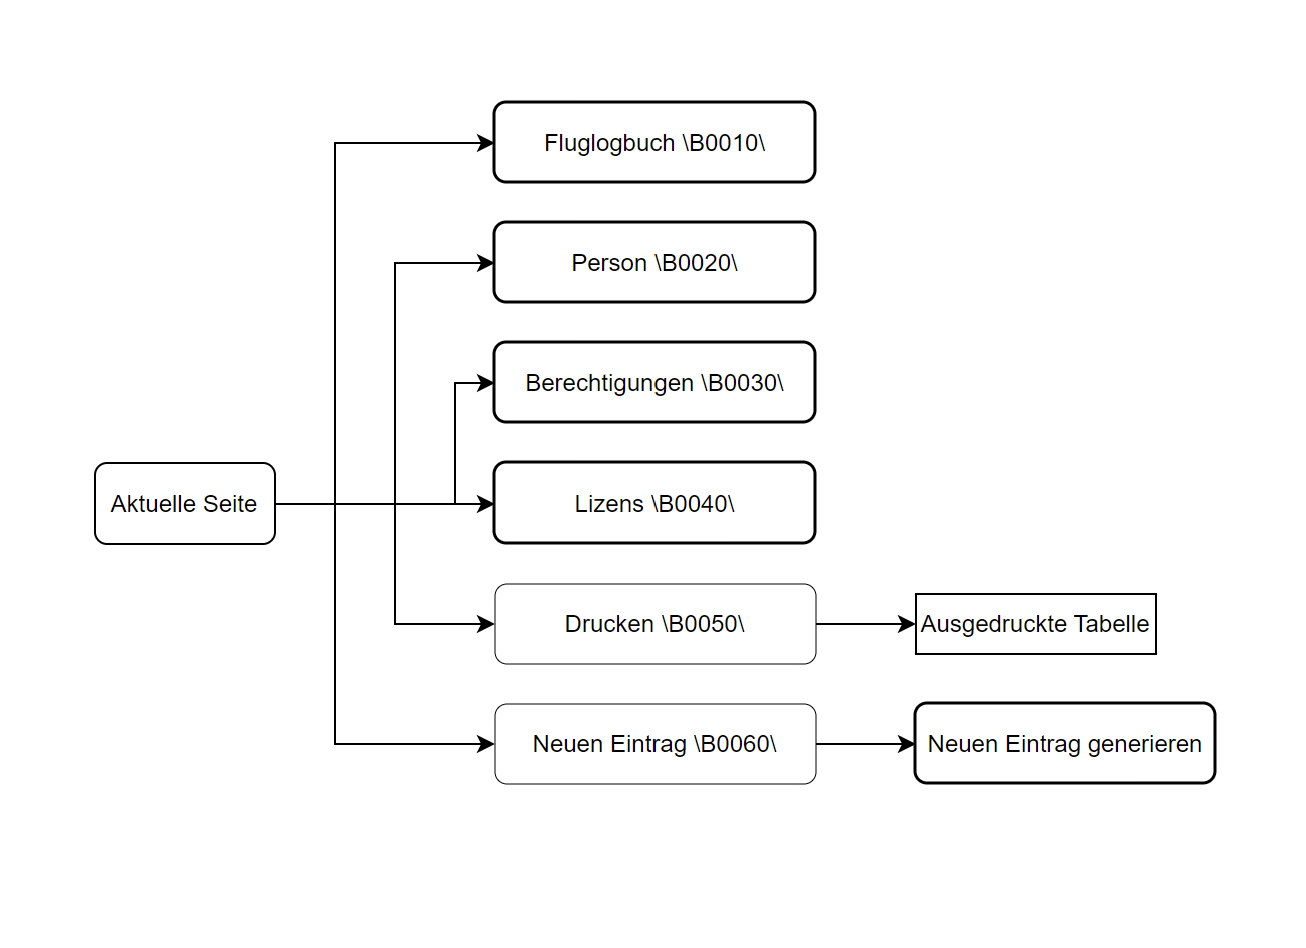
\includegraphics{Benutzeroberflaeche_Floglogbuch.png}
        \caption{Die Abbildung repräsentiert alle 4 Seiten}
        \label{fig:my_label}
    \end{figure}
    \pagebreak
    \subsubsection{Neuen Eintrag generieren}
    \vspace{0.5cm}
    Im folgenden ist der Aufbau der Seite \glqq{}Neuen Eintrag generieren\grqq{} modelliert.
    \begin{figure}[h!]
        \centering
        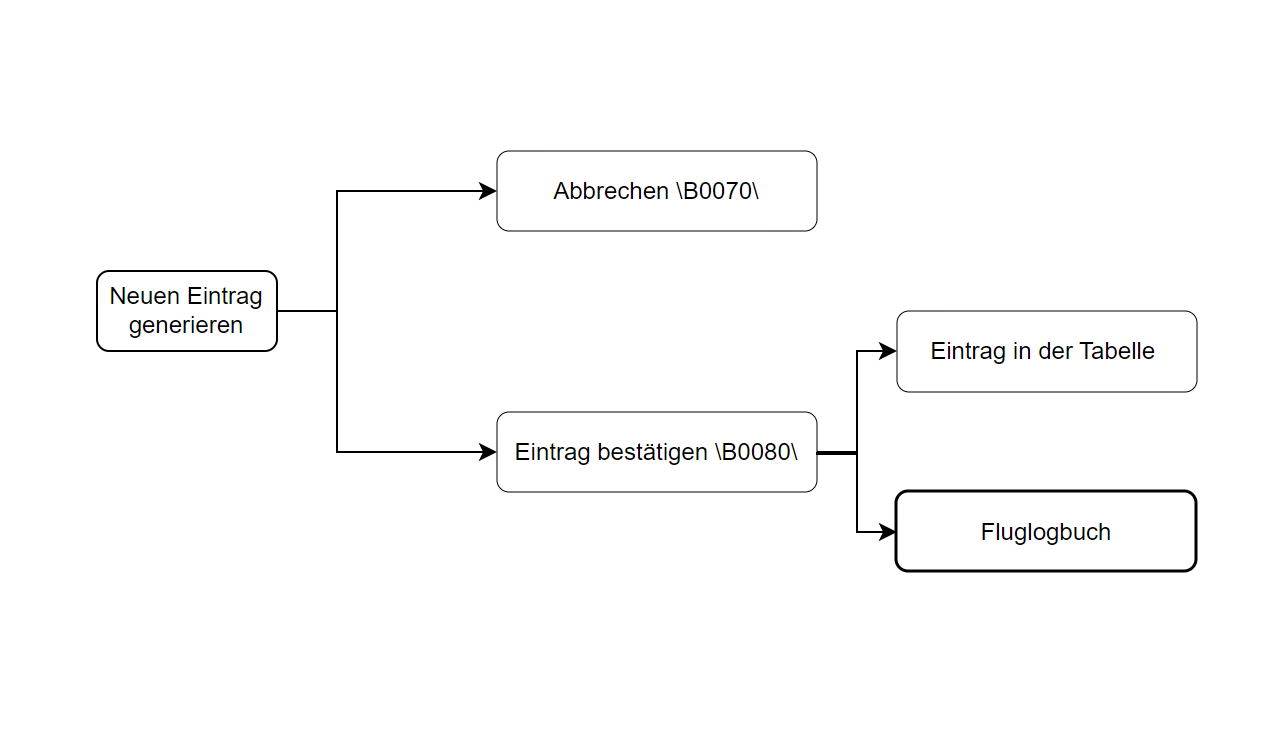
\includegraphics{Benutzeroberflaeche_Neuer_Eintrag.png}
        \caption{Neuen Eintrag generieren}
        \label{fig:my_label}
    \end{figure}
    
    \pagebreak

    \section{OOA-Modell}
    \begin{figure}[h]
        \centering
        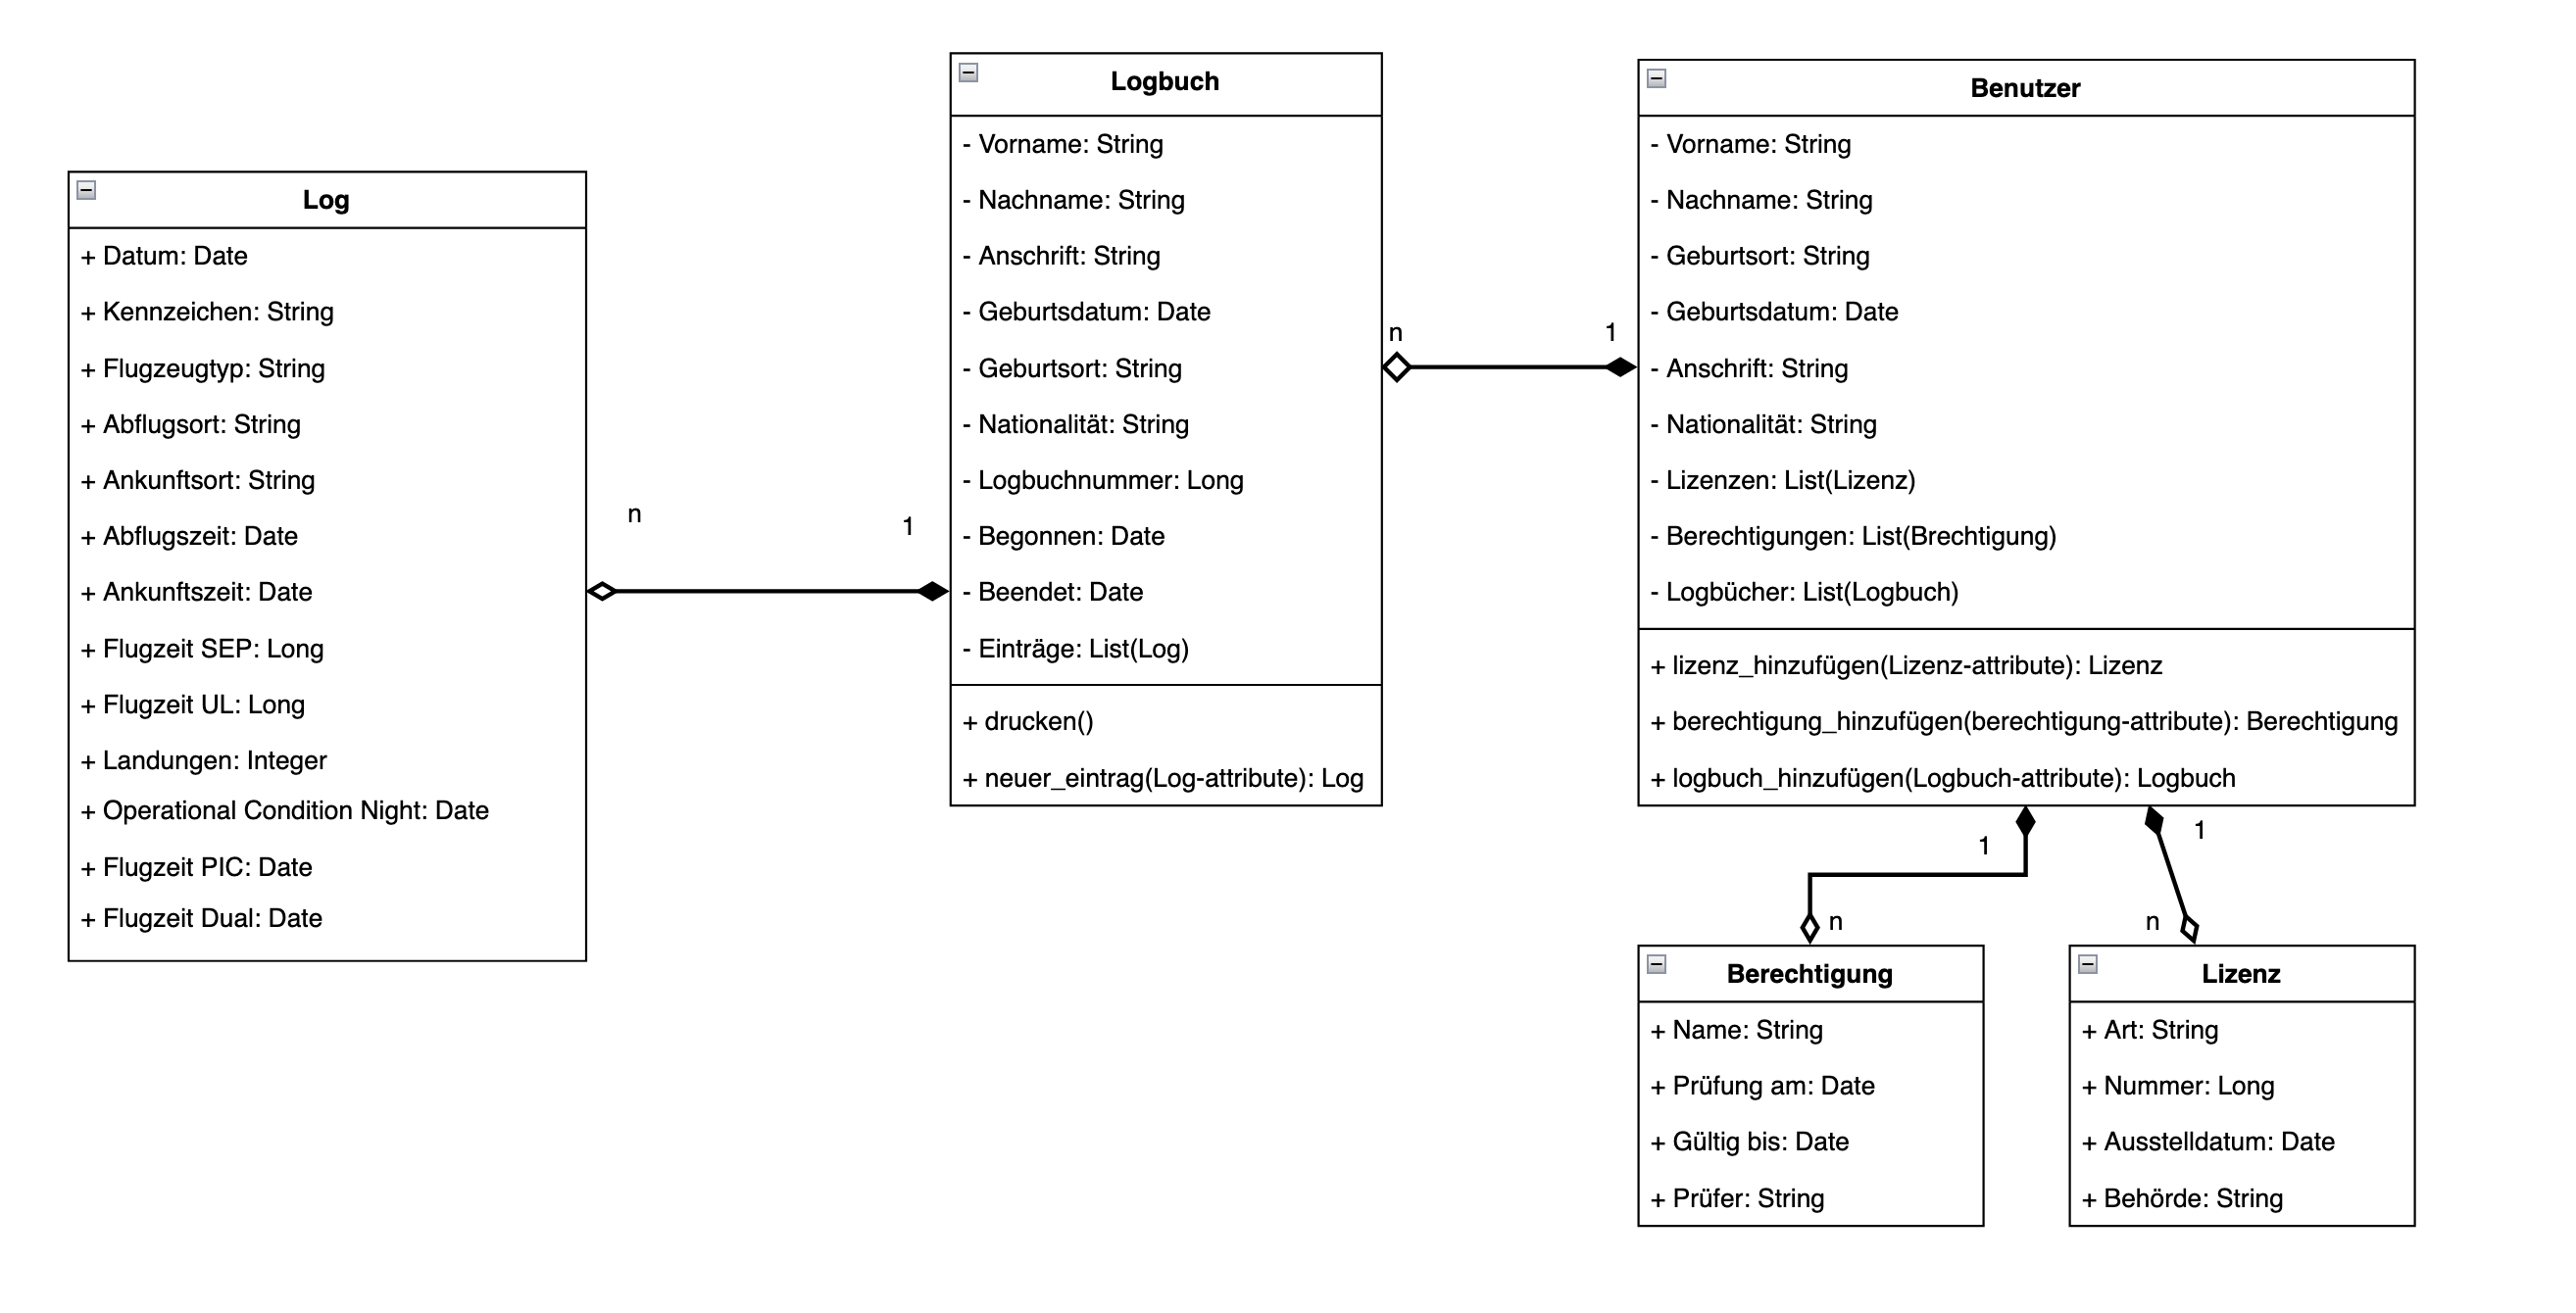
\includegraphics[width=18cm]{Abbildung_OOA.png}
        \label{fig:my_label}
    \end{figure}
    \pagebreak

    \section{Konzept der Benutzerschnittstelle}
    Text
    \pagebreak
    
    \section{OOD-Modell}
    Text/Bild
    \pagebreak

\end{document}